\documentclass[../../main.tex]{subfiles}
\begin{document}


{\bf [解]}
簡単のため $c=\cos\theta, s=\sin\theta$ と書く．
ただし
\begin{align}
 0 < \theta < \dfrac{\pi}{2} \label{eq:1}
\end{align}
である．

(1)
\begin{align}
  \begin{cases}
  0\le x\le c \\
  0\le y\le s
  \end{cases} \label{eq:2}
\end{align}
のもとで $Q(u,v)$ ($u=x+y, v=xy$) の軌跡をもとめる．
$c, s$の$\theta=\dfrac{\pi}{4}$に関する対称性からまず$0<\theta\le\dfrac{\pi}{4}$ で考える．
$u,v$ は $t$ の2次方程式 $t^2-ut+v=0$ の\cref{eq:2}をみたす2実解である．
$f(t)=t^2-ut+v$ とおく．$0<\theta\le\dfrac{\pi}{4}$ より $c\ge s$ だから\cref{eq:2}を満たすのは以下のいずれかである．

\begin{figure}[htb]
\begin{center}
  % --- 1° の場合 ---
  \begin{tikzpicture}[scale=1.2, >=stealth]
    % 軸
    \draw[->] (-0.4, 0) -- (2.2, 0) node[right] {$t$};
    \draw[->] (0, -0.6) -- (0, 1.3) node[above] {$y$};
    \node[below left] at (0,0) {$O$};

    % 放物線 y = f(t)
    \draw[thick, domain=-0.1:1.7, samples=100] plot (\x, {1.8*(\x-0.4)*(\x-1.0)});

    % 交点と軸上のラベル
    \fill (0.4, 0) circle (1.2pt);
    \fill (1.0, 0) circle (1.2pt);
    \node[below] at (0.4, 0) {$t_1$};
    \node[below] at (1.0, 0) {$t_2$};

    % 範囲の区切り (s, c)
    \draw[dashed] (1.3, -0.5) -- (1.3, 1.0);
    \draw[dashed] (1.7, -0.5) -- (1.7, 1.0);
    \node[below, font=\small] at (1.3, 0) {$s$};
    \node[below, font=\small] at (1.7, 0) {$c$};

    % 図の下のキャプション表記
    \node[below] at (0.9, -0.8) {\small $1^\circ\ 0 \le t \le s$ に2実解};
  \end{tikzpicture}
  \hspace{0.5cm}
  % --- 2° の場合 ---
  \begin{tikzpicture}[scale=1.2, >=stealth]
    % 軸
    \draw[->] (-0.4, 0) -- (2.2, 0) node[right] {$t$};
    \draw[->] (0, -0.6) -- (0, 1.3) node[above] {$y$};
    \node[below left] at (0,0) {$O$};

    % 放物線 y = f(t)
    \draw[thick, domain=-0.1:1.7, samples=100] plot (\x, {1.8*(\x-0.4)*(\x-1.3)});

    % 交点と軸上のラベル
    \fill (0.4, 0) circle (1.2pt);
    \fill (1.3, 0) circle (1.2pt);

    % 範囲の区切り (s, c)
    \draw[dashed] (0.85, -0.5) -- (0.85, 1.0);
    \draw[dashed] (1.7, -0.5) -- (1.7, 1.0);
    \node[below, font=\small] at (0.85, 0) {$s$};
    \node[below, font=\small] at (1.7, 0) {$c$};

    % 図の下のキャプション表記
    \node[below] at (0.9, -0.8) {\small $2^\circ\ 0 \le t \le s, s \le t \le c$ に1つずつ};
  \end{tikzpicture}
\caption{$1^\circ$，$2^\circ$の場合分けにおける$t$の範囲}
\end{center}
\end{figure}

\paragraph{1. $0\le t\le s$に2実解を持つ時}

$f(t)=0$ の判別式を $D$ とすると，この時の条件は
\begin{align}
  \begin{cases}
  D\ge0 \\
  f(0), f(s)\ge0 \\
  0\le \dfrac{u}{2}\le s
\end{cases}
\iff
\begin{cases}
  u^2-4v\ge0 \\
  0\le u\le 2s \\
  v\ge0 \\
  s^2-us+v\ge0
\end{cases} \label{eq:3}
\end{align}

\paragraph{2. $0\le t\le s,\ s\le t\le c$ に1つずつ解を持つ時}

この時の条件は
\begin{align}
  f(0)\ge0,\ f(s)\le0,\ f(c)\ge0
  \iff
  \begin{cases}
  v\ge0 \\
  s^2-us+v\le0 \\
  c^2-uc+v\ge0
  \end{cases} \label{eq:4}
\end{align}
である．

よって求める領域は\cref{eq:3}または\cref{eq:4}である．
$\dfrac{\pi}{4}\le\theta<\dfrac{\pi}{2}$ の時は $c$ と $s$ を入れかえれば良い．
これを図示して下図斜線部（境界含む）である．

\begin{figure}[htb]
\begin{center}
\begin{tikzpicture}[scale=3, >=stealth]
  % パラメータ設定 (0 < theta < pi/4 の例: theta = pi/6, s=0.5, c=0.866)
  \def\s{0.5}
  \def\c{0.866}

  % ========================================================
  % 塗りつぶし処理（2つの領域のOR）
  % ========================================================
  % 領域1: u ∈ [0, 2s] (放物線 v = 1/4 u^2 と u 軸の間)
  \fill[pattern=north east lines, pattern color=black!70] 
    plot[domain=0:{2*\s}, samples=50] (\x, {0.25*\x*\x}) 
    -- ({2*\s}, 0) -- (0,0) -- cycle;

  % 領域2: u ∈ [2s, s+c] (直線 v = su - s^2, 直線 v = cu - c^2, u 軸の間)
  \fill[pattern=north east lines, pattern color=black!70] 
    ({2*\s}, 0) 
    -- ({2*\s}, {\s*\s}) 
    -- ({\s+\c}, {\c*\s}) 
    -- ({\c}, 0) -- cycle;

  % ========================================================
  % 描画
  % ========================================================
  % 座標軸
  \draw[->] (-0.8, 0) -- (2.0, 0) node[right] {$u$};
  \draw[->] (0, -0.8) -- (0, 1.5) node[above] {$v$};
  \node[below left] at (0,0) {$O$};

  % 曲線・直線の描画（領域の境界線を強調）
  % 放物線 v = 1/4 u^2
  \draw[thick] plot[domain=0:{2*\s}, samples=50] (\x, {0.25*\x*\x});
  \draw[dashed, gray] plot[domain=0:-0.8, samples=50] (\x, {0.25*\x*\x}) node[above, color=black, font=\small] {$v = \frac{1}{4}u^2$};
  \draw[dashed, gray] plot[domain={2*\s}:2.2, samples=50] (\x, {0.25*\x*\x});

  % 直線 v = su - s^2
  \draw[thick, green!80!black] ({2*\s}, {\s*\s}) -- ({\s+\c}, {\c*\s});
  \draw[dashed, green!80!black] (-0.2, {-0.2*\s - \s*\s}) -- ({2*\s}, {\s*\s});
  \draw[dashed, green!80!black] ({\s+\c}, {\c*\s}) -- (2.0, {2.0*\s - \s*\s}) node[below, color=green!80!black, font=\small] {$v = su - s^2$};

  % 直線 v = cu - c^2
  \draw[thick, blue!80!black] ({\c}, 0) -- ({\s+\c}, {\c*\s});
  \draw[dashed, blue!80!black] (0.4, {0.4*\c - \c*\c}) -- ({\c}, 0);
  \draw[dashed, blue!80!black] ({\s+\c}, {\c*\s}) -- (2.0, {2.0*\c - \c*\c}) node[above, color=blue!80!black, font=\small] {$v = cu - c^2$};

  % 補助線（点線）
  \draw[dotted] (0, {\s*\s}) -- ({2*\s}, {\s*\s}) -- ({2*\s}, 0);
  \draw[dotted] (0, {\c*\s}) -- ({\s+\c}, {\c*\s}) -- ({\s+\c}, 0);
  \draw[thick] ({2*\s}, {\s*\s}) -- ({2*\s}, 0);

  % 頂点・交点
  \fill (0,0) circle (1pt);
  \fill ({2*\s}, {\s*\s}) circle (1pt);
  \fill ({2*\s}, 0) circle (1pt);
  \fill ({\s+\c}, {\c*\s}) circle (1pt);
  \fill ({\c}, 0) circle (1pt);

  % ラベル表記
  \node[below, font=\small] at ({\c}, 0) {$c$};
  \node[below, font=\small] at ({2*\s}, 0) {$2s$};
  \node[below, font=\small] at ({\s+\c}, 0) {$s+c$};

  \node[left, font=\small] at (0, {\s*\s}) {$s^2$};
  \node[left, font=\small] at (0, {\c*\s}) {$cs$};

  % 条件
  \node[above left] at (-0.2, 1.8) {$1^\circ\ 0 \le \theta < \pi/4$};

\end{tikzpicture}
\caption{$(u,v)$の軌跡の図示（斜線部）}
\label{fig:1}
\end{center}
\end{figure}

\begin{figure}[htb]
\begin{center}
\begin{tikzpicture}[scale=3, >=stealth]
  % パラメータ設定 (theta = pi/4 のとき)
  % s = c = sqrt(2)/2 ≒ 0.7071
  \def\s{0.7071}

  % ========================================================
  % 塗りつぶし処理（ u ∈ [0, sqrt(2)] ）
  % 放物線 v = 1/4 u^2、直線 v = (sqrt(2)/2)u - 1/2、u軸で囲まれた領域
  % ========================================================
  \begin{scope}
    % 放物線の下側でクリップ
    \clip (0,0) -- plot[domain=0:{2*\s}, samples=50] (\x, {0.25*\x*\x}) -- ({\s},0) -- cycle;
    % 直線の上側でクリップ（u軸より上の領域）
    \fill[pattern=north east lines, pattern color=black!70] 
      plot[domain=0:{2*\s}, samples=50] (\x, {0.25*\x*\x}) 
      -- ({2*\s},0) -- ({\s},0) -- (0,0) -- cycle;
  \end{scope}

  % ========================================================
  % 描画
  % ========================================================
  % 座標軸
  \draw[->] (-0.8, 0) -- (2.0, 0) node[right] {$u$};
  \draw[->] (0, -0.8) -- (0, 1.5) node[above] {$v$};
  \node[below left] at (0,0) {$O$};

  % 放物線 v = 1/4 u^2 (境界は実線、延長は破線)
  \draw[thick] plot[domain=0:{2*\s}, samples=50] (\x, {0.25*\x*\x});
  \draw[dashed, gray] plot[domain=-0.8:0, samples=50] (\x, {0.25*\x*\x});
  \draw[dashed, gray] plot[domain={2*\s}:2.2, samples=50] (\x, {0.25*\x*\x}) node[above right, color=black, font=\small] {$v = \frac{1}{4}u^2$};

  % 直線 v = (sqrt(2)/2)u - 1/2 (境界は実線、延長は破線)
  % 接点 (sqrt(2), 1/2) から u軸交点 (sqrt(2)/2, 0) までは実線
  \draw[thick] ({\s}, 0) -- ({2*\s}, {0.5});
  \draw[dashed, gray] (-0.2, {-0.2*\s - 0.5}) -- ({\s}, 0);
  \draw[dashed, gray] ({2*\s}, {0.5}) -- (2, {2*\s - 0.5}) node[right, color=black, font=\small] {$v = \frac{\sqrt{2}}{2}u - \frac{1}{2}$};

  % 補助線（点線）
  % 接点 (sqrt(2), 1/2) から各軸への補助線
  \draw[dotted] (0, {0.5}) -- ({2*\s}, {0.5}) -- ({2*\s}, 0);
 

  % 頂点・交点・接点
  \fill (0,0) circle (1pt);
  \fill ({\s}, 0) circle (1pt);
  \fill ({2*\s}, 0.5) circle (1pt);

  % ラベル表記
  \node[below, font=\small] at ({\s}, 0) {$\frac{\sqrt{2}}{2}$};
  \node[below, font=\small] at ({2*\s}, 0) {$\sqrt{2}$};
 
  \node[left, font=\small] at (0, 0.5) {$\frac{1}{2}$};
  \node[left, font=\small] at (0, 1) {$1$};

  % 左上の条件
  \node[above left] at (-0.2, 1.4) {$2^\circ\ \theta = \pi/4$};

\end{tikzpicture}
\caption{$(u,v)$の軌跡の図示（$\theta = \pi/4$ の場合）}
\label{fig:3}
\end{center}
\end{figure}


この領域の面積$S(\theta)$を$0<\theta\le\dfrac{\pi}{4}$ の時に考えよう．
この面積は以下のように3つの部分に分解して計算できる．
\begin{align}
S(\theta) &= 
  \left( \text{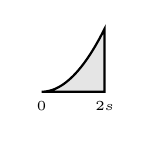
\begin{tikzpicture}[baseline={(0,-0.1)}, scale=0.8]
    % 放物線領域
    \fill[gray!20] (0,0) -- plot[domain=0:1] (\x, {\x*\x}) -- (1,0) -- cycle;
    \draw[thick] (0,0) -- plot[domain=0:1] (\x, {\x*\x}) -- (1,0) -- cycle;
    \node[below, font=\tiny] at (0,0) {$0$};
    \node[below, font=\tiny] at (1,0) {$2s$};
  \end{tikzpicture}} \right)
  + 
  \left( \text{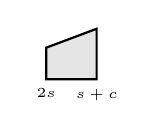
\begin{tikzpicture}[baseline={(0,-0.1)}, scale=0.8]
    % 台形/長方形領域
    \fill[gray!20] (0,0) -- (0,0.5) -- (0.8,0.8) -- (0.8,0) -- cycle;
    \draw[thick] (0,0) -- (0,0.5) -- (0.8,0.8) -- (0.8,0) -- cycle;
    \node[below, font=\tiny] at (0,0) {$2s$};
    \node[below, font=\tiny] at (0.8,0) {$s+c$};
  \end{tikzpicture}} \right)
  - 
  \left( \text{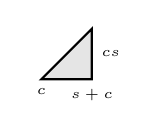
\begin{tikzpicture}[baseline={(0,-0.1)}, scale=0.8]
    % 三角形領域
    \fill[gray!20] (0,0) -- (0.8,0.8) -- (0.8,0) -- cycle;
    \draw[thick] (0,0) -- (0.8,0.8) -- (0.8,0) -- cycle;
    \node[below, font=\tiny] at (0,0) {$c$};
    \node[below, font=\tiny] at (0.8,0) {$s+c$};
    \node[right, font=\tiny] at (0.8,0.4) {$cs$};
  \end{tikzpicture}} \right) \\[2mm]
  &= \int_0^{2s} \frac{1}{4}u^2 \, du + \frac{1}{2}(c-s)(s^2+cs) - \frac{1}{2}c \cdot cs \\[2mm]
  &= \frac{2}{3}s^3 + \frac{1}{2}s(c^2-s^2) - \frac{1}{2}cs^2 \\[2mm]
  &= \frac{1}{6}s^3 + \frac{1}{2}sc^2 - \frac{1}{2}cs^2 \label{eq:5}
\end{align}
と計算できる．

次に$\theta=\dfrac{\pi}{4}$の時は\cref{fig:3}より同様に二つの部分から計算できて
\begin{align}
S(\theta) &= 
  \left( \text{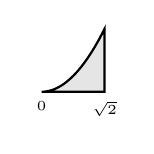
\begin{tikzpicture}[baseline={(0,-0.1)}, scale=0.8]
    % 放物線領域
    \fill[gray!20] (0,0) -- plot[domain=0:1] (\x, {\x*\x}) -- (1,0) -- cycle;
    \draw[thick] (0,0) -- plot[domain=0:1] (\x, {\x*\x}) -- (1,0) -- cycle;
    \node[below, font=\tiny] at (0,0) {$0$};
    \node[below, font=\tiny] at (1,0) {$\sqrt{2}$};
  \end{tikzpicture}} \right)
  - 
  \left( \text{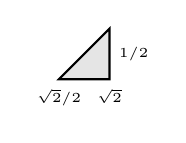
\begin{tikzpicture}[baseline={(0,-0.1)}, scale=0.8]
    % 三角形領域
    \fill[gray!20] (0,0) -- (0.8,0.8) -- (0.8,0) -- cycle;
    \draw[thick] (0,0) -- (0.8,0.8) -- (0.8,0) -- cycle;
    \node[below, font=\tiny] at (0,0) {$\sqrt{2}/2$};
    \node[below, font=\tiny] at (0.8,0) {$\sqrt{2}$};
    \node[right, font=\tiny] at (0.8,0.4) {$1/2$};
  \end{tikzpicture}} \right) \\[2mm]
 &=\int_0^{\frac{\sqrt2}{2}}\frac{1}{4}u^2du - \frac{1}{2}\cdot\frac{\sqrt2}{2}\cdot\frac{1}{2} \\
 &=\frac{\sqrt2}{24} \label{eq:6}
\end{align}
でこれは \cref{eq:5}に $\theta=\dfrac{\pi}{4}$ を代入したものにひとしい．

また $\dfrac{\pi}{4}<\theta<\dfrac{\pi}{2}$ の時は対称性から$s$ と $c$ を入れかえれば良い．
以上をまとめて求める面積$S(\theta)$は
\begin{align}
  S(\theta)=
  \begin{cases}
  \dfrac{1}{6}s^3+\dfrac{1}{2}sc^2-\dfrac{1}{2}cs^2 & \left(0<\theta\le\dfrac{\pi}{4}\right) \\[2mm]
  \dfrac{1}{6}c^3+\dfrac{1}{2}s^2c-\dfrac{1}{2}sc^2 & \left(\dfrac{\pi}{4}\le \theta\le\dfrac{\pi}{2}\right)
  \end{cases}
\end{align}
である．


(2)
(1)での議論の通り，$S(\theta)$は$\theta \to \dfrac{\pi}{2}-\theta$に対する入れ替えに対して対称であるから題意は示された．
数式的には(1)の結果で$0<\theta<\dfrac{\pi}{4}$ とすると
\begin{align*}
  S\left(\frac{\pi}{2}-\theta\right) = \frac{1}{6}s^3+\frac{1}{2}cs^2-\frac{1}{2}cs^2 = S(\theta)
\end{align*}
であるから示される．

\newpage

\end{document}
